
\section{Premessa}
Prima di proseguire con la lettura del documento è bene puntualizzare alcune cose.
Innanzitutto va ricordato che il nostro prodotto consta di 2 plugin distinti che svolgono funzioni diverse. Per semplificare la rappresentazione grafica e per evitare ripetizioni essi sono stati, in questa fase di progettazione, considerati come facenti parte dello stesso sistema. Questo è reso possibile dall'alta sovrapposizione di componenti necessari al loro funzionamento. Tuttavia, nella fase finale di produzione, essi verranno completamente disaccoppiati e saranno presentati come due plugin distinti che avranno delle parti in comune, che per come è progettato Kibana, dovranno essere per forza ripetute.\\
Come seconda cosa va segnalato che il linguaggio di programmazione da noi usato, Javascript, è weakly typed. Questo comporta. ad esempio, poca precisione per quanto riguarda il tipaggio dei parametri passati ai metodi. Per questo, soprattutto nella fase di rappresentazione grafica del sistema, ci terremmo vaghi sul tipo dei parametri passati e ritornati da metodi. Tali imprecisioni verranno tuttavia chiarite nella parte di testo che riguarda ogni specifico componente.

\section{Componenti}

Ogni plugin per Kibana è articolato in due sezioni principali: lato client e lato server. Si presenta di seguito il dettaglio di ciasuna sezione.

\subsection{Lato Server}
Il lato server si deve occupare di interrogare il database Elasticsearch ed esporre i risultati delle query tramite API REST al lato client.
\subsubsection{Rappresentazione}
Nel seguente diagramma delle classi, figura \ref{img:diagrammaClassiServer}, ciascuna API viene rappresentata tramite una classe composta da un singolo metodo. Tale metodo intende rappresentare il funzionamento della API.


\begin{figure}[h]
	\centering
	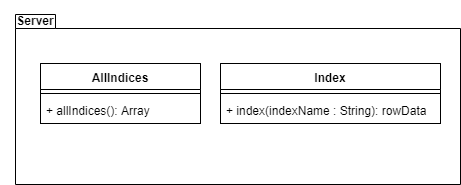
\includegraphics[width=1\textwidth]{Images/DiagrammaClassiServer.png}
	\caption{Diagramma UML delle classi riguardanti il lato server}
	\label{img:diagrammaClassiServer}
\end{figure}

\subsubsection{AllIndices}
AllIndices è la API che si occupa di restituire al chiamante la lista di \emph{tutti} gli indici presenti all'interno della istanza di Elasticsearch collegata. La lista degli indici è un array di stringhe contenente per ogni indice il proprio nome.

\subsubsection{Index}
Index è la API che espone l'interfaccia per poter leggere i dati contenuti all'interno di un indice. Nella richiesta GET deve essere specificato un parametro chiamato index, il cui valore rappresenta l'indice del quale si vogliono ottenere i dati. Ciò che viene ritornato al richiedente è un oggetto \emph{grezzo}, ovvero la risposta dell'istanza Elasticsearch, con tutti i metadati che Elasticsearch utilizza annessi. Sarà compito del client reperire le informazioni a lui utili

\subsection{Lato Client}
Il lato client si occupa di interrogare il lato server per ottenere informazioni grezze, elaborarle per renderle utili ed infine presentarle all'utente.

\label{sec:Componenti}
\subsubsection{Rappresentazione}
Il codice prodotto è stato scritto in Javascript ES6, quindi molti concetti quali classi ed interfacce non sono presenti all'interno del linguaggio. Per produrre un diagramma delle classi dunque sono state considerate \emph{ classi } sia oggetti Javascript, sia funzioni. Per quanto riguarda le interfacce che sono presenti nel diagramma delle classi, figura \ref{img:diagrammaClassiClient}, nel codice non sono effettivamente presenti tali interfacce, ma tutte le classi che implementano tale interfaccia \emph{devono} possedere i metodi esposti da tale interfaccia. Questo stratagemma è stato particolarmente utile nell'implementazione del componente \texttt{DataCleaner}, come descritto in \ref{sec:DataCleaner}

\begin{figure}[H]
    \centering
    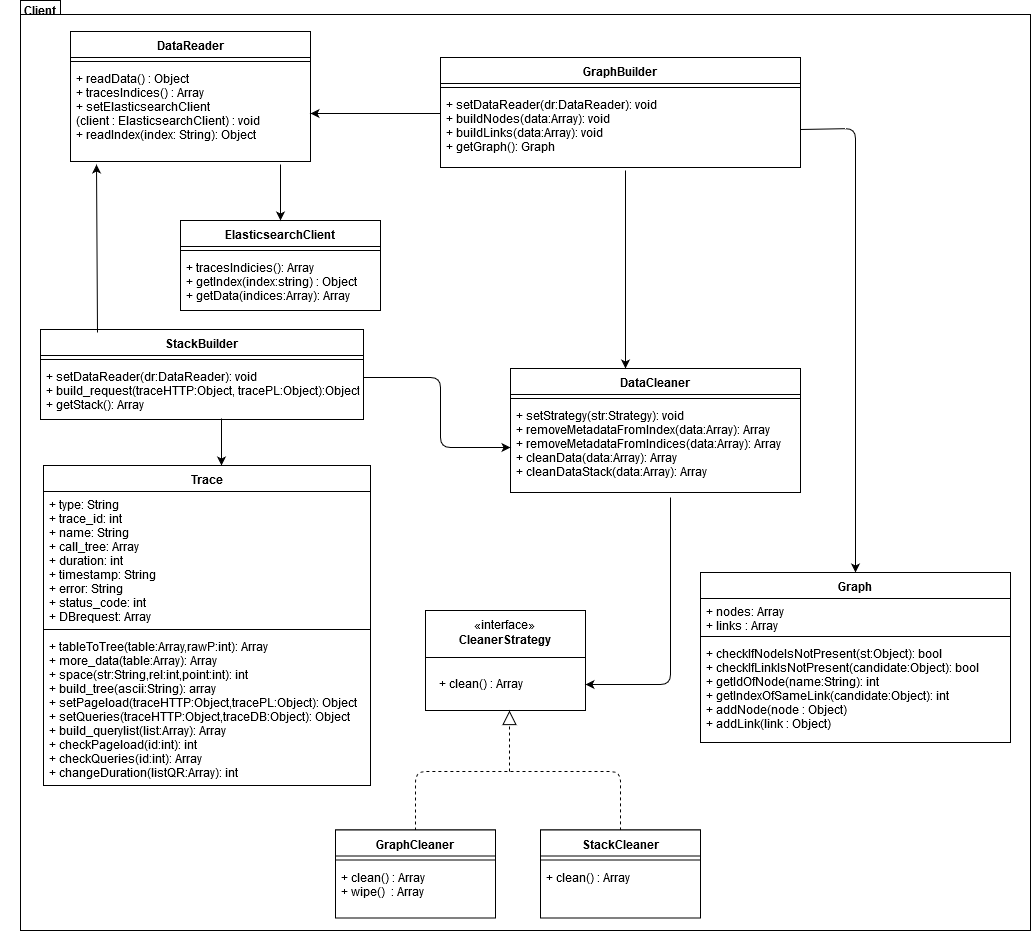
\includegraphics[width=1\textwidth]{Images/classi.png}
    \caption{Diagramma delle classi dell'applicazione}
    \label{img:diagrammaClassiClient}
\end{figure}

\subsubsection{ElasticsearchClient} 
\texttt{ElasticsearchClient} è il componente che si occupa di fare le chiamate API al lato server. Non è una classe vera e propria all'interno del codice, ma un \emph{Service}. 
I Service sono funzioni, od oggetti, che possono essere passati a tutte le altri componenti di angularJs attraverso Dependency Injection, permettono di condividere codice e funzionalitá facilmente. Essi sono lazily instantiated, cioé generati solo quando un componente esprime una dipendenza verso un determinato service e realizzano il design pattern "singleton", rendendoli particolarmente efficenti ed adatti per la realizzazione di servizi come i client API, dove avere piú istanze dello stesso client non sarebbe ragionevole.
Utilizzare un service è l'unico modo per poter eseguire chiamate REST parametrizzate al lato server. I metodi da esso esposti sono: 
\begin{itemize} 
  \item \texttt{tracesIndices()} ritorna un array di stringhe che rappresenta gli indici contenuti nell'istanza di ElasticSearch che hanno all'interno delle traces; 
  \item \texttt{getIndex(index)} ritorna al chiamante i dati grezzi che vengono restituiti da Elasticsearch eseguendo una ricerca priva di parametri sull'indice passato come parametro, ovvero \texttt{index}. Essi comprendono, oltre tutti i documenti dell'indice, anche i metadati di Elasticsearch; 
  \item \texttt{readData()}: ritorna al chiamante un array di dati grezzi, ognuno dei quali rappresenta il risultato di una ricerca priva di parametri su un indice. Gli indici letti sono quelli ritornati da \texttt{tracesIndices()}, ovvero tutti e soli quelli che contengono traces. 
\end{itemize} 
Osserviamo che anche se in questa rappresentazione questi metodi sono all'interno di un oggetto, non avendo i diagrammi delle classi UML un costrutto per rappresentare precisamente un \emph{service}, essi non hanno una struttura ben definita e oggetti di tipo \texttt{ElasticsearchClient} chiaramente non sono istanziabili. Dunque, per interfacciarsi ad Elasticsearch si è deciso di racchiudere tutte queste funzionalità in un oggetto vero e proprio, \texttt{DataReader} (descritto nella sezione \ref{sec:DataReader}), per poter avere una più agevole interazione con i dati. 
 

\subsubsection{DataReader}
\label{sec:DataReader}
\texttt{DataReader} è il componente del sistema che si occupa di reperire i dati da Elasticsearch, tuttavia ciò viene fatto utilizzando il \emph{service} \texttt{ElasticsearchClient}. Sarebbe effettivamente possibile utilizzare le chiamate al \emph{service} ogni qualvolta fossero necessari dei dati, tuttavia ricordiamo che tali chiamate non vengono racchiuse all'interno di un oggetto ben strutturato, ma sono un \emph{service}. Restituirà ai richiedenti le informazioni grezze, esattamente come vengono restituite da Elasticsearch. I metodi sono: 
 

\begin{itemize}
	\item \texttt{setElasticsearchClient(client)}: permette di impostare una sorgente dei dati;
	\item \texttt{tracesIndices()}: ritorna un array di stringhe, i quali elementi sono tutti e soli gli indici all'interno dell'istanza di Elasticsearch che hanno al loro interno delle traces. Ciò viene realizzato tramite una chiamata al lato server all'API \texttt{AllIndices} e dunque vengono tenuti solo indici che contengono nel nome la sottostringa \emph{spans};
	\item \texttt{readIndex(index)}: ritorna al chiamante i dati grezzi che vengono restituiti da Elasticsearch eseguendo una ricerca priva di parametri sull'indice passato come parametro, ovvero \texttt{index}. Essi comprendono oltre tutti i documenti dell'indice anche i metadati di Elasticsearch;
	\item \texttt{readData(indices)}: ritorna al chiamante un array di dati grezzi, ognuno dei quali rappresenta il risultato di una ricerca priva di parametri su un indice. Gli indici letti sono quelli passati tramite parametro.


\end{itemize}



\subsubsection{DataCleaner}

\label{sec:DataCleaner}
\texttt{DataCleaner} è il componente del sistema che si occupa di pulire i dati grezzi che sono stati reperiti da ElasticSearch. Esso compie questo lavoro in due momenti: prima estraendo i dati "utili" da Elasticsearch e poi pulendoli attraverso una \emph{strategy}, descritta in \ref{sec:CleanerStrategy}.\\
Il metodo \texttt{clean(data)} si occupa di realizzare ciò.
Per estrarre i dati utili esso si avvale di un metodo, \texttt{removeMetaData(data)}, il quale si occupa di rimuovere i metadati di Elasticsearch che sono presenti quando si prelevano i dati. Questo metodo ritorna un array contenente i documenti JSON così come essi sono stati inseriti dall'applicazioni di monitoring negli indici di ElasticSearch. ElasticSearch, infatti, immagazzina i documenti JSON nel campo \texttt{\_source} il quale è inserito in oggetti che contengono altri dati ed informazioni "di servizio". Il metodo si occupa di rimuovere questi dati e costruisce un array contenente il solo contenuto dei campi \texttt{\_source}. Il client che utilizza questa classe comunque in generale ha la necessità di ripulire ulteriormente i dati dei documenti, per esempio eliminando certi tipi di trace (ad esempio tenere solamente traces di richieste HTTP). Per poter soddisfare ogni richiesta specifica un \texttt{DataCleaner} contiene un oggetto che rispetti l'interfaccia \texttt{CleanerStrategy}. La strategy viene incaricata di raffinare ulteriormente i dati per la costruzione della Mappa Topologica oppure per la costruzione dello Stack Trace tramite il metodo \texttt{clean(data)}. \\
Risulta chiaro che esiste dunque una dipendenza fra la struttura dei dati che vengono restituiti da ElasticSearch, la classe \texttt{DataCleaner} e le classi che implementano \texttt{CleanerStrategy}. Tuttavia, i client di \texttt{DataCleaner} potranno avere accesso diretto ai dati di ElasticSearch, privi di dati amministrativi.

	
\subsubsection{CleanerStrategy}
\label{sec:CleanerStrategy}

\texttt{CleanerStrategy} è l'interfaccia che verrà implementata per realizzare una pulizia più raffinata dei dati di un \texttt{DataCleaner}. Espone il metodo \texttt{clean(data)}, che avrà comportamenti diversi a seconda della strategia che si desidera applicare. Dato che il prodotto è implementato in Javascript il costrutto interfaccia non è presente nel linguaggio. Per ovviare a questa mancanza tutte le classi che dovrebbero implementare questa interfaccia \emph{devono} possedere un metodo \texttt{clean(data)} che funzioni come ci si aspetti. 

	
	
\subsubsection{GraphCleaner}
\label{sec:GraphCleaner}

\texttt{GraphCleaner} è l'implementazione di \texttt{CleanerStrategy} utilizzata da \texttt{DataCleaner} per pulire i dati che dovranno essere utilizzati per la costruzione del grafo rappresentante la mappa topologica. Il metodo \texttt{clean(Array)}, che riceve in input un Array di indici che contengono al loro interno i documenti JSON sottoforma di Array. Tale metodo agisce scorrendo l'array che riceve invocando il metodo \texttt{wipe(Array)} su ogni sottoarray. Il metodo \texttt{wipe(Array)} ha come output esclusivamente l'insieme di documenti all'interno dell'indice che rappresentano richieste di dati ai database dell'applicazione oppure ai server, ovvero il sottoinsieme di documenti che serviranno effettivamente per la costruzione del grafo.
	
\subsubsection{StackCleaner}
\label{sec:StackCleaner}

\texttt{StackCleaner} è l'implementazione di \texttt{CleanerStrategy} utilizzata da \texttt{DataCleaner} per pulire i dati che dovranno essere utilizzati durante la costruzione della stack trace. Essa dispone del metodo \texttt{clean(data)} il quale scorre tutti i documenti JSON disponibili e ha come output l'insieme di documenti che rappresentano chiamate HTTP, JDBC oppure Pageload, ovvero tutte e sole quelle necessarie per la costruzione dei dati strutturati della stack trace.



\subsubsection{StackBuilder}
\label{sec:StackBuilder}

\texttt{StackBuilder} si occupa della riorganizzazione dei dati e della loro elaborazione in modo da ottenere una struttura dati ottimale per la successiva visualizzazione della Stack Trace.\\
Esso viene istanziato con un oggetto \texttt{DataReader} per poter ottenere i dati.
Il metodo principale è \texttt{getStack()} che controlla tutte le chiamate HTTP ricevute dal \texttt{DataReader} e pulite dal \texttt{DataCleaner}, creato e istanziato con strategia \texttt{StackCleaner}. \texttt{GetStack()} riorganizza i dati in base alla loro tipologia che viene identificata tramite i metodi \texttt{checkPageload()} e \texttt{checkQueries()} per poter essere successivamente mostrati in modo più agevole. Le tipologie di richieste possono essere:
	\begin{itemize}
		\item HTTP: insieme di metodi scatenati da un evento generico;
		\item HTTP + Pageload: insieme di metodi scatenati dal caricamento di una pagina web;
		\item HTTP + JDBC + Pageload: insieme di eventi che portano all'interrogazione di un database e che provocano un successivo caricamento di una pagina.
	\end{itemize}
	Per ognuna di queste è costruita una struttura dati che seleziona solo i campi del JSON ricevuto da \texttt{StackCleaner()} veramente utili alla generazione della stack trace.
	In particolare i dati che devono essere presenti in tutte le tre tipologie  sono:
	\begin{itemize}
		\item \texttt{type}: che riconduce ad una delle tre tipologie di trace;
		\item \texttt{trace\_id}: numero univoco che permette l'associazione tra trace HTTP, JDBC e Pageload;
		\item \texttt{name}: identificazione generale della richiesta;
		\item \texttt{call\_tree}: array contenente gerarchicamente la lista dei metodi invocati dall'applicazione per compiere la richiesta;
		\item \texttt{duration}: tempo impiegato dal sistema per lo svolgimento della richiesta, compreso il tempo dei metodi, delle query e del caricamento della pagina;
		\item \texttt{timestamp}: data e ora dello svolgimento della richiesta;
		\item \texttt{error}: presenza o meno di errori;
		\item \texttt{status\_code}: tipologia di errore.
	\end{itemize}
	Questi dati vengono ulteriormente manipolati per essere visualizzati in maniera conveniente nella Stack Trace.  \\
	Il metodo \texttt{change\_duration} permette di far variare il tempo di esecuzione delle richieste in base alla tipologia in quanto per ognuna bisognerà considerare più parametri per calcolare i millisecondi impiegati.\\
	Per il campo \texttt{call\_tree} avviene un'accurata manipolazione attraverso il metodo \texttt{build\_tree()} per passare da un tipo stringa ad una gerarchia di oggetti.
	 Al metodo \texttt{build\_tree()} viene passato il dato sotto forma di stringa in cui, attraverso l'ASCII art, viene rappresentato un albero dei metodi che vengono invocati con delle informazioni particolari per ognuno di essi. Questo utilizza a sua volta il metodo \texttt{more\_data()} per costruire un array bidimensionale che elenca tutti i metodi e per ognuno ne specifica i dati aggiuntivi rappresentati dall'ASCII art (come total time e self time), il grado di indentazione nell'albero, il numero di metodi figli e il numero di metodi discendenti da esso. \\ Da questa struttura il metodo \texttt{tableToTree()} ricava un oggetto con innestati altri oggetti rappresentanti i metodi e i propri dati strutturati in maniera da rispecchiare i legami di parentela dell'ASCII art.


\subsubsection{GraphBuilder}
\label{sec:GraphBuilder}
	\texttt{GraphBuilder} è il componente che si occupa di costruire il grafo di nodi e archi rappresentanti la mappa topologica dell'applicazione. Esso verrà successivamente visualizzato utilizzando la libreria D3.js. \texttt{GraphBuilder} viene istanziato con un oggetto \texttt{DataReader} per poter ottenere i dati di cui ha bisogno.
	Il metodo principale è \texttt{getGraph()} che costruisce il grafo partendo dai dati letti dal \texttt{DataReader}. Quando si invoca tale metodo, viene costruito il \texttt{DataCleaner} con strategia \texttt{GraphCleaner} e i dati grezzi vengono letti e successivamente ripuliti dai relativi componenti.
	I metodi \texttt{getNodes(Array)} e \texttt{getLinks(Array, Array)} vengono utilizzati per poter completare la costruzione del grafo.\\
	Il metodo \texttt{getNodes(Array)} costruisce l'insieme di nodi che faranno parte della mappa topologica. Esso scorre tutti i documenti JSON preparati dal \texttt{GraphCleaner} che gli vengono passati come input ed a seconda della tipologia di chiamata (a Database oppure a Server) crea un oggetto candidato ad entrare nell'insieme dei nodi. Il fatto che tale candidato non sia già presente nell'insieme dei nodi viene garantito dal metodo \texttt{checkIfNotPresent(Object)}.
	Il metodo \texttt{getLinks(Array, Array)} invece, costruisce l'insieme di collegamenti che ci saranno tra i nodi del grafo. Un link tra due nodi è caratterizzato dai seguenti campi:
	\begin{itemize}
		\item{\texttt{source}, che rappresenta il nodo che ha effettuato la chiamata sotto forma di id numerico intero;}
		\item{\texttt{target}, che rappresenta il nodo che ha ricevuto la chiamata sotto forma di id numerico intero;}
		\item{\texttt{type}, che può essere "Database" o "HTTP", per rappresentare i diversi tipi di comunicazione;}
		\item{\texttt{average\_response\_time}, che contiene il tempo medio di risposta di tutte le trace tra source e target;}
		\item{\texttt{number\_of\_requests}, che serve per mantenere consistente il campo \texttt{average\_response\_time}.}
	\end{itemize}
	Ogni collegamento è individuato univocamente dalla coppia \texttt{source} e \texttt{target}.
	Il metodo scorre tutti i documenti JSON che gli vengono passati come array e per ogni documento, che contiene la trace di una comunicazione tra due componenti dell'applicazione costruisce un oggetto candidato ad entrare nell'insieme. Il fatto che tale link candidato non sia già presente nell'insieme viene garantito dal metodo \texttt{checkIfLinkIsNotPresent(Array, Object)} che controlla che nell'array dei links non sia già presente un collegamento con gli stessi campi \texttt{source} e \texttt{target} del candidato. Se non esiste un collegamento con quei campi \texttt{source} e \texttt{target} ne viene inserito uno nuovo, altrimenti ci si limita ad aggiornare i campi \texttt{average\_response\_time} e \texttt{number\_of\_requests} tenendo conto dei nuovi dati. 

\section{Visualizzazione delle informazioni}

\subsection{Mappa topologica}

\subsection{StackTrace}
	Il (rendering)GLOSSARIO dello stack si avvale delle numerose direttive fornite da
angularJs.


Data la natura complessa che dati che devono essere rappresentati, sono state
implementate delle direttive personalizzate angularJs.
Le direttive (in inglese directives) sono dei marcatori di elementi del DOM che permettono di allegare
a tali elementi e ai loro figli comportamenti specifici attraverso il complier
HTML di AngularJs.

Esse sono  caratterizzate da
	\begin{itemize}
		\item nome
		\item parametri di configurazione
		\item scope:  che rappresenta una reference ai dati, siano essi array, oggetti o
				semplici variabili, che la direttiva utilizza per generare l'html
		\item template html
		\item funzione: che permette di rendere piú complesso il comportameto della direttiva
					e di riempire il template hmtl con i dati ricevuti
	\end{itemize}

La vera potenza delle direttive risiede nel fatto che sono innestabili tra loro,
ovvero una direttiva puó, al suo interno, richiamare un'altra direttiva. Ció
rappresenta la soluzione perfetta per i tipi di dato che trattiamo noi, in quanto
hanno tutti una struttura ricorsiva (array di array per la maggior parte).

Le direttive, al loro interno, oltre ad utilizzare altre direttive scritte da noi,
utilizzano quelle native di angularJs. Ció permette di generare l'html molto
facilmente. Per esempio tra le direttive built-in piu utili fornite da angular sono:
\begin{itemize}
	\item ngFor: permette di iterare su una collezione di elementi
	\item ngIf: applicare una classe css al verificarsi di una condizione
	\item ngController: assegna un controller ad una view
\end{itemize}

Per renderizzare la nostra stack trace sono state create due direttive.
\begin{itemize}
	\item branch la quale si occpua di generare dell' html per ogni oggetto che gli viene passato,
  		in branch viene inoltre specificata la funzione link che permette di gestire un caso particolare
 	\item tree il cui compito di interare sugli oggetti di un array. Per ogni elemento iterato viene richiamata
  		la direttiva branch.
\end{itemize}

Nel direttive vengono infine richiamate nel codice HTML semplicemente creando un
tag con lo stesso nome della direttiva, infatti le direttive permettono di creare
tag personalizzati che vengono poi interpretati dall'parser di angularJs.
Nel nostro caso, le direttive vengono usate per popolare la tabella delle stack trace
e per ogni trace la corrispondente sotto tabella consentendo di riutilizzare il codice
molto efficacemente.



\section{Interazioni fra componenti}
\label{sec:Interazioni}
Qui diagrammi di sequenza

\section{Tracciamento dei requisiti}
\label{sec:Tracciamento}
Qui swego 
